%\documentclass{article}
\documentclass[10pt, conference, compsocconf]{IEEEtran}

\usepackage{graphicx}
\usepackage{subfig}
\usepackage{url}
\usepackage{algorithm}
\usepackage{algorithmic}
\usepackage{listings}
\usepackage{amsmath}
\usepackage{amsthm}
\usepackage{verbatim}
\graphicspath{{./figures/}{./simulation/}{../figures/psware/}{../simulation/psware/}}
\newcommand{\HRule}{\rule{\linewidth}{0.5mm}}
%\newcommand{\figurecurrentwidth}{\includegraphics[width=\textwidth]}
%\newcommand{\figurehalfwidth}{\includegraphics[width=.5\textwidth]}
\newcommand{\figurecurrentwidth}{\includegraphics[width=.49\textwidth]}
\newcommand{\figurehalfwidth}{\includegraphics[width=.24\textwidth]}
\lstset{float, numbers=left, frame=lines, belowcaptionskip=3mm, xleftmargin=7mm, framexleftmargin=7mm, escapeinside={(*}{*)}, tabsize=3, breaklines=true}
\newtheorem{theorem}{Theorem}
\renewcommand{\algorithmicrequire}{\textbf{Input:}}
\renewcommand{\algorithmicensure}{\textbf{Output:}} 
\pdfminorversion=9

\begin{document}

\title{PSWare: A Flexible Middleware Framework for Composite Event in Wireless Sensor Network}
\author{
{Scribus Primus}\\
\affaddr{Primus Address}\\
\email{primus@somewhere.com} \and
{Scribus Secundus}\\
\affaddr{Secundus Address}\\
\email{secondus@elsewhere.com}
}
\conferenceinfo{SenSys'11,} {November 1--4, 2011, Seattle, WA, USA.}
\CopyrightYear{2011}
\crdata{XXX-X-XXXXX-XXX-X}
\maketitle
\begin{abstract}
Event detection is an important topic in many WSN applications. Although there are several works on providing event-based services in WSN, most of them can only deal with primitive event types but cannot handle composite events very well. In general, a type-based event system may have primitive or composite event types. All event types are defined by specifying their attributes and filters. Then, individual events are detected and delivered according to such type information. Composite event types may be defined by combining multiple event types with operators. Due to the resource constraints in WSN, composite events are much more difficult to manage than primitive events. In this work, we introduce PSWare, a type-based publish / subscribe middleware for WSN that supports composite events. We describe our design for PSWare. PSWare has a flexible architecture where different composite event detection algorithms may be easily integrated.

On top of PSWare, we present TED (Type-based Event Detection), a novel distributed composite event detection algorithm. The essential idea of TED is event fusion, where some sensor nodes are selected as fusion points and component events are fused for the detection of a high level event. Event fusion with minimum energy cost is an NP-complete problem. Therefore, TED uses a number of heuristics with bounded performance.  

To further increase the performance of event detection, we design a clustering algorithm for PSWare for structural health monitoring applications (SHM). We formulate the problem and found it to be NP-complete so we propose heuristic centralized and distributed algorithms. In addition to SHM, We use PSWare to develop other real world WSN applications including intelligent transportation system (ITS) and in-door monitoring.

We evaluate our system from different aspects. We first evaluate TED, the most essential algorithm in our system. We analyze its performance and then carry out extensive simulations. Both analytical and simulation results show TED can save energy in event-based applications where primitive events occur in a higher frequency than composite events. Then we combine TED with PSWare and carried out some real world experiments. The results show that PSWare can offer reasonably simple API for the application developers to use while TED and our clustering algorithm can improve the underlying event detection performance. Compared with opportunistic approaches to event detection in these real applications, PSWare can reduce 40 - 50 \% of the energy cost.
\end{abstract}
\chapter{Introduction}
\section{Overview}
\label{sec:introduction}
Development in wireless communication and electronics has made it possible to create low-cost, low-power wireless sensor nodes. Each sensor node usually contains a wireless transceiver, a micro processing unit and a number of sensors. The sensor nodes can collect data and do some simple processing locally, and can communicate with each other to form an ad hoc wireless sensor network (WSN) \cite{aky:survey}. A WSN is usually self-organized and self-maintained without any human intervention. Wireless sensor networks have been used in various application areas such as smart building \cite{lynch:shm}, wild environment monitoring \cite{wsnhabitat}, intelligent transportation systems \cite{klein:its}, battle surveillance \cite{wsntracking} and healthcare \cite{lo:ban}. 

While WSN has a wide range of applications, programming sensor networks is a challenging because different from programming in the traditional environment. WSN imposes a lot of constraints such as limited computational power, less memory and unreliable communication. Application developers need to not only understand the requirements for the specific application domain but also take into consideration of the characteristics of WSN. In this research work, we propose PSWare, a publish/subscribe (pub/sub) middleware for WSN which eases the development of WSN applications. Our middleware uses a pub/sub programming paradigm for the application programmer to subscribe application specific events. It provides an easy-to-use Event Definition Language (EDL) to allow the application developers to define composite events while uses a flexible architecture so that different domain-specific event processing algorithms can be easily integrated into the middleware.

\subsection{Motivation}
Despite the large variety of WSN applications, many of them are essentially event-based. In applications such as intelligent transportation systems \cite{klein:its}, smart buildings \cite{lynch:shm} and healthcare \cite{lo:ban}, the events sensor nodes detect events which reflect the environmental changes and the systems respond to these events accordingly. Events may be primitive or composite. Primitive events (e.g. when the temperature exceeds certain threshold) can be detected by a single sensor node without having to cooperate with others. On the other hand, \emph{composite events} consist of multiple primitive events. They reflect a serial of environmental changes with spatial and temporal relations among them and must be detected collaboratively by different sensor nodes.

Because of the common requirements and challenges for composite event subscription and detection, it is more desirable to have a generic middleware layer to handle composite events instead of reinventing the wheel and implementing application-specific event processing mechanisms. In addition, the middleware should be flexible enough so that different event processing algorithms for different application domains can be easily integrated. In summary, the middleware should achieve the following design goals:
\begin{enumerate}
\item \emph{Event abstraction}: since composite events are collaboratively processed by different sensor nodes in the network, they introduce extra complexity because of the resource constraints and unreliable communication. A middleware framework providing high level event abstraction is needed to ease the application development.
\item \emph{Re-usability and flexibility}: different applications may share certain common modules during event processing. They may also have other different modules. A middleware framework can help so that common modules may be used and different modules may be replaced without affecting others.
\end{enumerate}

\subsection{Issues}
In this research, we address the essential issues of designing and developing PSWare. On the highest level, an event description language is provided to allow users to describe composite event relationships. On the lowest level, a runtime environment is necessary on each sensor nodes so that they could understand and execute the event processing algorithms translated from the high-level EDL. More specifically, we need to address the following research/engineering issues to make our middleware work.

\begin{itemize}
\item	\emph{Event definition language}: we need to provide an event description language which is powerful yet easy to use.
\item	\emph{Event definition language compiler}: a compiler is essential to translate the programs written in our high-level language into a low-level language understandable by the sensor nodes. The compiler must be smart enough to extract the semantic meanings from the program and do some optimization.
\item	\emph{Runtime environment support}: the middleware running on each sensor node should provide a runtime environment to execute the compiled programs.
\item	\emph{Subscription propagation}: after the program written in EDL is compiled, the subscription should be intelligently disseminated into the network. If the subscription is too big, it may need to be divided into small ones. Furthermore, only related sensor nodes need to be updated.
\item	\emph{Event detection}: we need to design efficient protocol for the sensor nodes to cooperate with each other to detect composite events.
\item	\emph{Event delivery}: after the subscribed the events have been detected, we need energy-efficient routing protocols so that the detected events will be delivered at the minimum cost.
\end{itemize}
\section{Related Works}
\label{sec:relatedworks}
Existing works on pub/sub systems for WSN primarily consider the detection of primitive events where each event is usually treated separately and events don't have relations between each other. \cite{lowlevelnaming} is a pub/sub system built on top of directed diffusion \cite{directeddiffusion}. The sink node will first broadcast interest and the source nodes will deliver the detected events through gradients and reinforced paths. Mires \cite{mires} is a pub/sub middleware for WSN. It makes use of the message-oriented communication paradigm provided by TinyOS \cite{nesc}. First, nodes will advertise their available topics using a multi-hop routing protocol. Then, the sink will broadcast the subscription and finally, nodes will be able to publish the events to the sink. \cite{sp} had an in-depth discussion on the trade-off between reliability and energy consumption. Instead of flooding the subscription to every node in the network, the flood stops after certain number of hops. If the subscription does not reach the publisher, then the event will be forwarded probabilistically. 

More recently, certain works such as \cite{lai:ted, complexevent} have been proposed for composite event definition and detection. The primary focus of \cite{lai:ted} is on a composite event detection algorithm called TED which utilizes event type information for efficient detection. In addition to an event language, \cite{complexevent} also discusses how to reliably detect composite events in a pervasive environment. The focus of this paper is on a flexible middleware framework so that different event detection algorithms may be integrated and evaluated easily.

Apart from the pub/sub paradigm, there have been a lot of efforts on developing other type of programming abstractions for WSN including query-based approaches \cite{cougar, sina, tinydb} VM-based approaches \cite{magnetos, mate, smartmessage} tuple space-base approaches \cite{tinylime} neighbor-based approach \cite{kairos, hood, abstractregion} and mobile agent-based approaches \cite{agilla, sensorware}.

In terms of composite event detection in WSN, there have been very limited works. However, a lot of work has been done on data aggregation for sensor network. Existing data aggregation can be mainly divided into three categories: cluster-based approach \cite{leach, iheed, epas}, chain-based approach \cite{pegasis} and tree-based approach \cite{mfst, dctc, tag, xue:lp, tina}. Cluster-based approach typically considers the problem how to select and rotate cluster heads so that the clusters can be evenly distributed in the network \cite{iheed} and energy consumption will be balanced \cite{leach}. Cluster-based approach can be organized into multiple levels in order to further save the cost. Chain-based approach improves cluster-based approach by letting each sensor node only communicate with its close neighbors \cite{pegasis}. Tree-based approaches have many differnt optimizatin techniques. For example, \cite{xue:lp} formulates the problem as a multi-commodity flow problem and uses linear programming to solve it.  MFST \cite{mfst} constructs a minimum Steiner tree with a cost model that considers the fusion cost. 

We believe the pub/sub paradigm is suitable for many WSN applications because many of these applications are event-based in nature. However, more work needs to be done in order to support efficient composite event detection, especially how to support application-specific event detection mechanisms so that high energy efficiency can be achieved.
\floatname{algorithm}{Algorithm}
\chapter{Composite Event Detection}
\label{chapter:ted}
\section{The Composite Event Detection Problem}
\label{sec:system_model}
Event detection algorithm is the heart of a pub/sub system. In this section, we formally define the composite event detection algorithm.

\subsection{System Model}
We consider the network as a graph \(G=(N, A)\) where each node represents a sensor node and each edge represents a communication link. For each \(a_n\in A\), it has a weight \(W_n\) associated with it.

The subscriber provides a finite set of event types \(E=\{e_1,e_2,\cdots\}\). For each \(e_n\in E\), the subscriber defines a set of attributes \(e_n\rightarrow attr_n\) which reflect certain real world phenomenon. 

The subscriber also provides a finite set of event relations \(R=\{r_1,r_2, \cdots\}\) where each \(r_n\in R\) represents the mapping of one or more sub-event types \(e_1, e_2\cdots \in E\) to a composite event type \(e_3\in E\), denoted as \(r_n(e_1, e_2, \cdots)=e_3\). One of the event type \(e_s\in E\) is subscribed by the subscriber. %Event types and their relations can be represented as a directed acyclic graph (DAG) as shown in Figure \ref{fig:eventdag}, where each node represents an event and each edge represents a relation between a sub-event and a composite event.

\begin{comment}
\begin{figure}
\centering
\figurecurrentwidth{eventdag}
\caption{Event DAG}
\label{fig:eventdag}
\end{figure}
\end{comment}

We have a set of primitive event types \(E_{primitive}\subseteq E\) event types such that \(\not{\exists} r_n\in R\) such that \(r_n(e_1, e_2, \cdots)=e_n\) where \(e_n\in E_{primitive}\) and \(e_1, e_2, \cdots \in E\). For each primitive event of type \(e'_n\in E_{primitive}\), it will be detected by a node \(n_i\in N\). We use the message cost as the event detection cost for each event type \(e_n\in E\), denoted as \(cost(e_n)\).

\subsection{Problem Formulation}
Given:
\begin{itemize}
	\item A network \(G=(N, A)\)
	\item A set of event types \(E\) with relation \(R\)
	\item A cost function \(cost(e_n)\) for \(e_n\in E\)
\end{itemize}

Find:
\begin{itemize}
	\item For each event type \(e_n\in E\), when an event instance of this type is happens, find a subset of nodes \(V_n^r\subseteq V\) which are involved in detecting the event.
\end{itemize}

Objective:
\begin{itemize}
	\item Minimize the total energy consumption:
	\begin{displaymath}
	\sum_{i=i}^{n}cost(e_i)
	\end{displaymath}
\end{itemize}

\begin{theorem}
\label{thm:tableConstruction}
The composite event detection problem is NP-complete.
\end{theorem}

\begin{proof}
We show our proof by reducing the steiner tree problem to our composite event detection problem. Let \(N_s\subset N\) be the event source (nodes that detect the primitive events). Since the cost is defined as message cost, if we minimize the total path length from the event sources to the fusion points (nodes which are responsible for detecting composite events), then we can also minimize the message cost.

We construct a graph \(G'=(N', A')\) from \(G\) with the steps as follows:
\begin{enumerate}
\item \(N'=N_s\bigcup N_f\)
\item For each pair of nodes \(n'_i, n'_j\in N'\), we add an edge \(a'_k\in A'\) incident on both if there is a path from \(n'_i\) to \(n'_j\) in \(G\).
\item The weight of the newly added edge is \(a'_k\) is the weight of the shortest path from \(n'_i\) to \(n'_j\) in \(G\).
\end{enumerate}

The corresponding Steiner tree problem can be defined as below.

Given:
\begin{itemize}
\item A graph: \(G'=(N', A')\)
\item Each edge \(e'_i\) in the graph has a weight of \(W'_i\)
\item A set of sources: \(N_s\subset N\)
\end{itemize}

Find:
\begin{itemize}
\item A minimum Steiner tree that spans \(N_s\)
\end{itemize}

If we have a solution for the Steiner tree problem in \(G'\), then we simply need to recover the shortest paths in \(G\) and it will also be the optimal solution for our composite event detection problem. On the other hand, an optimal solution for our composite event detection problem is also an optimal solution for the Steiner tree problem if we replace the paths between every pair of nodes \(n'_i, n'_j\in N'\)  with the edges in \(A'\).
\end{proof}

\section{Fully distributed TED}
\label{sec:cedu}
In this section, we introduce TED, a distributed type-based composite event detection algorithm for WSN. The essential idea of TED is that after each sub-event is detected, the nodes will at first forward the detected events randomly to some nearby fusion points in the hope that at least some of them will be able to detect events at lower cost. When the composite events are detected, the fusion points will first check to see if the source nodes have already selected any fusion point. If not, it will flood some feedback in the network so that the source node will get it and other nodes can also use such feedbacks as 'hints' when they need to forward the events. By collecting different feedbacks from different fusion points, the sensor nodes will choose the best one according to the cost. If the sub-events occur again, the nodes will be able to forward the detected events based on the feedback so that the cost could likely be reduced.

\subsection{Algorithm Input}
In TED, the set of event fusion points \(N_f\subseteq N\) are preselected. We will discuss how to select the fusion points in an optimal way in the latter part of the section. Therefore, each node will play two possible roles: normal node or event fusion point. Normal nodes will need the following data structure for the algorithm:
\begin{itemize}
\item Event filter table \(table_f\): this table stores the filters for each event type. \(table_f\rightarrow filter_n\) denotes the filter for event type \(e_n\).
\item Fusion point routing table (\(table_r\)): this table defines the routing to each fusion point \(n_i\in N_f\). \(table_r\rightarrow n_i\rightarrow parent\) denotes the parent node to reach fusion point \(n_i\).
\item Event forwarding table (\(table_e\)): this table defines for each event type \(e_n\in E\), the corresponding fusion point for the it. \(table_e\rightarrow e_n\rightarrow fp\) denotes the fusion point for event type \(e_n\).
\end{itemize}

The fusion points will also have the same data structure of the normal nodes for the algorithm. In addition, they will have an additional table \(table_m\). This table temporarily stores the events collected from other nodes. For each of the entries it has the following contents: 
\begin{itemize}
\item \(e^i_n\): the \(i^{th}\) event of type \(e_n\)
\item \(cost\): the detection cost for the event \(e^i_n\)
\item \(flag\): the flag (to be described in the algorithms) for the event \(e^i_n\)
\end{itemize}

\subsection{TED for Normal Nodes}
Since the event detection starts from primitive events, the normal nodes will run Algorithm \ref{algo:normalNode} after detecting a primitive event \(e^i_n\) of type \(e_n\).
\begin{algorithm}
\begin{algorithmic}
\REQUIRE evaluate(\(e^i_n\), \(table_f\rightarrow filter_n\))==True
	\IF {\(table_e\rightarrow e_n\rightarrow flag\neq fpUnknown\)}
		\STATE \(toForward=table_e\rightarrow e_n\rightarrow fp\)
		\STATE Set \(e^i_n\rightarrow flag=table_e\rightarrow e_n\rightarrow flag\)
		\STATE Forward \(e^i_n\) to \(table_r\rightarrow fp\rightarrow parent\)
	\ELSE
		\IF{\(table_e\rightarrow e_n\rightarrow flag\neq fpUnknown\)}
			\STATE Select \(k-1\) nearest fusion points \(N_k\in N_f\)
			\STATE \(N_k=N_k\bigcup \{table_e\rightarrow e_n\rightarrow fp\}\)
		\ELSE
			\STATE Select \(k\) nearest fusion points \(N_k\in N_f\)
		\ENDIF
		\FOR {each \(n\in N_k\)}
			\STATE forward \(e^i_n\) to \(table_r\rightarrow n\rightarrow parent\)
		\ENDFOR
	\ENDIF
	
	\IF {\(e^i_n\rightarrow flag=fpSelected\) \AND \(e^i_n\rightarrow timeout==True\)}
		\STATE \(table_e\rightarrow e_n\rightarrow flag=fpIndicated\)
	\ENDIF
\REQUIRE feedback of event type \(e_n\) from \(n_i\in N_f\)
	\STATE \(entry=table_e\rightarrow e_n\)
	\IF {\(e_n\rightarrow source==self\) \AND (\(entry\rightarrow flag\neq fpSelected\) \OR \(entry\rightarrow flag==fpSelected\) \AND \(entry\rightarrow cost<e_n\rightarrow cost\))}
		\STATE \(entry\rightarrow flag=fpSelected\)
		\STATE \(entry\rightarrow fp=n_i\)
	\ELSIF {\(entry\rightarrow cost<e_n\rightarrow cost\)}
		\STATE \(table_e\rightarrow e_n\rightarrow flag=fpIndicated\)
	\ENDIF
\end{algorithmic}
\caption{TED for normal nodes}
\label{algo:normalNode}
\end{algorithm}
For each event type, it has three possible states: fpUnknown, fpIndicated and fpSelected. Initially, all the event types are fpUnknown because the sensor node does not know which fusion point is the best to forward the event. The flag will be updated upon the reception of feedbacks from the fusion points. More specifically, if the event is detected at the fusion point \(n_i\), the fusion point will flood the feedback with cost and event source included so that the nodes can update their corresponding flags. The update is based on the detection cost.

Upon the detection of event \(e^i_n\), the node will first check if there is already a fusion point assigned to it. If so, the event will simply be forwarded to that fusion point. Otherwise, the node will choose \(k\) closest fusion points randomly and then forward the events to them.

\subsection{TED for Event Fusion Points}
When the fusion point receives \(e^i_n\) from a node, it will first wait a period of time until the expiry time of the event to check for other events for possible matches. If no match is found during this period, the fusion point will still use Algorithm \ref{algo:normalNode} to further forward the events to other fusion points. The pseudo code is shown in Algorithm \ref{algo:fusionPoint}.

\begin{algorithm}
\begin{algorithmic}
\REQUIRE \(e^i_n\) from node \(n_i\in N\)
	\FORALL {\(e_j\in E\)}
		\IF {\(e_n\) is a subevent of \(e_j\)}
			\STATE result = evaluate \(e_j\) with \(e^i_n\)
			\IF {result==True}
				\STATE detected (\(e_j\))
				\STATE \(e_j\rightarrow cost=e_j\rightarrow cost+e^i_n\rightarrow cost\)
				\STATE \(e_j\rightarrow source=e_j\rightarrow source\bigcup e^i_n\rightarrow source\)
				\STATE feedback (\(e_j\))
			\ENDIF
		\ENDIF
	\ENDFOR
\REQUIRE expiry time of \(e^i_n\)
	\STATE detected (\(e_j\))
\end{algorithmic}
\caption{TED for fusion points}
\label{algo:fusionPoint}
\end{algorithm}

The function 'detected' is the place where Algorithm \ref{algo:normalNode} is invoked. Upon the detection of any composite event, the fusion point will also send the feedbacks to the network.

\subsection{Determine the Re-selection Probability}
While the previous sections outline the algorithm for TED, we still need to decide how often the nodes should switch to another fusion point in order to cope with the event dynamics and network topological changes. We use exponential distribution as the event probability distribution because of its memoryless property. More specifically, for each composite event, the distance between each of its sub-events to any point in the network follows an exponential distribution as follows:
\begin{displaymath}
f(x)={\lambda}_1e^{-{\lambda}_1x}
\end{displaymath}

In addition to the distance between events, the direction of events that happen in different rounds will also affect the selection probability. The angle between any pair of related events also satisfy an exponential distribution as follows:
\begin{displaymath}
f(\theta)={\lambda}_2e^{-{\lambda}_2\theta}
\end{displaymath}

Both \(x\) and \(\theta\) are shown in Figure \ref{fig:event-distribution1} where the events \(e_1\), \(e_2\) are detected before and \(e'_1\), \(e'_2\) are detected. For simplicity, we use distance to measure the cost for one node to reach another. Let \(d\) be the average distance between any point in the deployment region to the closest sensor node. As shown in Figure \ref{fig:fp-dist}, for a composite event that has two sub-events, originally the event is fused at \(n_1\). Then, for the next detection of \(e'_1\) and \(e'_2\), if the fusion point is still the original one, then the cost will be no less than:
\begin{align*}
cost_1=\sqrt{({\lambda}_1)^2+(\frac{{\lambda}_1}{2})^2+({\lambda}_1)^2cos(\frac{\pi+{\lambda}_2}{2})}
\end{align*}
On the other hand, if a new fusion point is selected, then the cost will be no more than:
\begin{align*}
cost_2=&2(\frac{{\lambda}_1}{2sin\frac{{\lambda}_2}{2}}+{\lambda}_1)sin\frac{{\lambda}_2}{2}+d\\
=&{\lambda}_1(1+2sin\frac{{\lambda}_2}{2})+d
\end{align*}

\begin{figure}
\centering
\subfloat[Event distribution]{\label{fig:event-distribution1}\figurehalfwidth{event-distribution1}}
\subfloat[Fusion point distance]{\label{fig:fp-dist}\figurehalfwidth{fp-dist}}
\caption{Fusion points selection}
\label{fig:centralizedCEDU}
\end{figure}

The condition to select a new fusion point will be:
\begin{align}
&cost_1\geq cost_2\nonumber \\
&cost_1^2\geq cost_2^2\nonumber \\
&({\lambda}_1)^2(\frac{5}{4}+cos(\frac{\pi+{\lambda}_2}{2})\geq\nonumber \\ &{\lambda}_1^2(1+2sin\frac{{\lambda}_2}{2})^2+d^2+2{\lambda}_1(1+2sin\frac{{\lambda}_2}{2})d
\label{eq:fpSwitch}
\end{align}

Here \(d\) is decided by the node density and can be estimated once we know the deployment area and the number of nodes in the deployment area. Therefore, given \(f(x)\), \(f(\theta)\) and \(d\), we can use certain numeric methods such as generalized gradient search to find the values for \(\theta\) and \(x\) such that Equation \ref{eq:fpSwitch} is satisfied while minimizing the probability for switching:
\begin{align*}
P_{switch}&=F(x>x*)F(\theta>\theta *)\\
&=\int_{x*}^{\infty}{\lambda}_1e^{-{\lambda}_1x}dx\int_{\theta *}^{\infty}{\lambda}_2e^{-{\lambda}_2\theta}d\theta\\
&=e^{-{\lambda}_1x*}e^{-{\lambda}_2\theta *}
\end{align*}

Once the probability is obtained, after each event detection, there will be a probability of \(P_{switch}\) that the event will switch to another fusion point. This is done by making the fusion point broadcast a message in the network so that all nodes can delete the corresponding event type assignment to that fusion point.

\subsection{Fusion Point Deployment}
Because our distributed algorithm is based on certain nodes in the network that acts as event fusion points to detect the events, in this section, we discuss how to select such fusion points in order to efficiently detect the events. To give an answer without losing generality, we use the following deployment model:
\begin{itemize}
\item The entire network is divided into a set of equally sized regions.
\item Within each region, we deploy the same number of event fusion points. 
\end{itemize}

Such deployment model is suitable if the user has no prior knowledge on where the events would happen. After calculating the optimal deployment strategy, the users can make use of it in two ways:
\begin{itemize}
\item Even deployment: after the sensor deployment, the users can deploy additional sensor nodes as fusion points in the network.
\item Random deployment: before the deployment, the user can calculate how many fusion points are needed in the network and mix them with normal nodes to deploy them randomly.
\end{itemize}

We will use square for calculating the optimal deployment strategy in this paper. The optimal deployment strategies with regions of other types of shape may be also be obtained in a similar fashion. Suppose we divide the whole region of area \(A\) into squares of size \(s\times s\). Then on average, each sensor node can find a fusion point at a distance of:
\begin{align}
r=&\int_0^1D(t)dt\nonumber\\
=&\int_0^1\frac{2}{3}\sqrt{c^2t^2+(b^2-a^2-c^2)t+a^2}dt\nonumber\\
=&\frac{c}{6}[u(1+v^2)+\frac{1}{2}(1-u^2)(1-v^2)ln(\frac{u-1}{u+1})]\label{eq:avgdist1}
\end{align}
where,
\begin{align}
c=&\frac{s}{2}\nonumber\\
u=&\frac{\sqrt{2}+1}{2}s\nonumber\\
v=&\frac{\sqrt{2}-1}{2}s\label{eq:avgdist2}
\end{align}

In order to determine the optimal deployment strategy, we also need to know the event probabilistic distribution. We use the same exponential distribution model as above. %We start by considering the simplest case where two sub-event types \(e_1\) and \(e_2\) form a composite event type \(e_3\) (\(r_n(e_1, e_2)=e_3\)). 

The cost introduced by TED mainly consists of three parts: forwarding cost, feedback cost and detection cost. Initially, upon the detection of primitive events, the nodes will randomly forward the events to \(k\) closest fusion points. 
\begin{displaymath}
cost_{forward}=r\times k
\end{displaymath}

Here \(k\) is determined by the event distribution such that after forwarding different sub-events to the fusion points, there may be some overlapping fusion points for different sub-events. Therefore, \(k\) is defined as follows:
\begin{equation}
k=(\frac{{\lambda}_1}{r}+1)^2\label{eq:forwardNum}
\end{equation}

When the events are detected at the fusion points, feedback will be sent to the event sources so that the sensor nodes can later forward the events to them and the cost will be reduced. For simplicity of analysis, we assume the fusion points will simply flood the feedback in the network. Therefore, the feedback cost is:
\begin{displaymath}
cost_{feedback}=|N|\times k
\end{displaymath}

The detection cost is the message cost for all sub-events to be forwarded to a fusion point so that the composite event may be detected. If we have two events \(e_1\) and \(e_2\), the minimum event detection cost will be detecting the events on the line segment that connects the two events. However, we may not find a fusion point on the line segment, so in order to find a fusion point that can minimize energy cost, we should choose a point that lies on the bisector of the line segment (the detailed proof is omitted for brevity). Similar to Equation \ref{eq:avgdist1} and \ref{eq:avgdist2}, the average detection cost will be:
\begin{displaymath}
cost_{detect}=2\times \int_0^{arctan\frac{2r}{{\lambda}_1}}\frac{{\lambda}_1}{2cosx}dx
\end{displaymath}

Since each node needs to know how to reach the fusion points when forwarding is needed, there is overhead for maintaining such information. Similar to many existing routing protocols for WSN, we assume the nodes will periodically send messages for link evaluation \cite{rssiroute}. Therefore, the cost for maintenance is:
\begin{displaymath}
cost_{maintenance}=(\frac{A}{s^2})|N|c_1
\end{displaymath}

Here, \(c_1\) is constant that represents the relation between energy consumption and the size of the packets. In addition, the sensor node should also have storage constraint because the nodes simply might not able to store all the routes to every fusion point. The storage constraint is defined as:
\begin{displaymath}
(\frac{A}{s^2})<c_2
\end{displaymath}

Objective is to minimize:
\begin{displaymath}
cost_{all}=2(\frac{T}{t}+1)cost_{forward}+cost_{maintenance}+Tcost_{detect}
\end{displaymath}

All the constants are summarized in Table \ref{tab:ceduConstants}. \(cost_{all}\) may be obtained by nonlinear programming techniques such as generalized gradient search algorithm. In addition to square deployment, other deployment method may also be used and the only difference lies in Equation \ref{eq:avgdist1}, \ref{eq:avgdist2} and \ref{eq:forwardNum}.

\begin{table}
\begin{center}
\begin{tabular}{ | p{1cm} | p{5cm} | }
\hline
\({\lambda}_1\) & Expected location between the events \\ \hline
\({\lambda}_2\) & Expected angle of the events \\ \hline
\(A\) & Deployment area \\ \hline
\(s\times s\) & The size of the square sub-regions \\ \hline
\(c_1\) & Energy cost per bit of data transmission\\ \hline
\(c_2\) & Storage constraint\\ \hline
\end{tabular}
\end{center}
\caption{Summary of the symbols in TED}
\label{tab:ceduConstants}
\end{table}


\section{Evaluation}
\label{sec:ceduevaluation}
\begin{comment}
In this section, we evaluate the performance of TED through analysis, simulation and experiments.
\end{comment}
\subsection{Analysis}
\label{sec:ceduanalysis}
In order to analyze the energy efficiency of TED without losing generality, we assume the sensor nodes are randomly deployed in a circular area with radius of \(R\). We use distance to approximately measure the number of hops in order to calculate the message cost for event detection. As a reference to compare the energy cost, we use shortest path tree (SPT) algorithm where the events are collected at the sink because their definitions are not considered for the event detection.

We use a similar event model that has been introduced in Section \ref{sec:cedu} for analysis. Moreover, since the actual cost of TED will depend on event probabilities. We include such information in our model as well. Suppose we have two event types \(e_1\) and \(e_2\) which are the two sub-event types for a composite event \(e_3\) (i.e. \(e_1re_2=e_3, r\in R\)). The probability for \(e_1\) and \(e_2\) to occur is \(P(e_1)=p_1\) and \(P(e_2)=p_2\) respectively. The probability for \(e_3\) to occur when both \(e_1\) and \(e_2\) have occurred is \(P(e_3|e_1, e_2)=p_3\).

In TED, each node periodically broadcasts its routes to the fusion tables so that others can know how to reach the fusion points. Such cost is similar to many existing routing protocols in WSN such as \cite{rssiroute} where each node periodically broadcasts its route metrics to the sink for the purpose of link quality evaluation. Therefore, in TED, we mainly consider three parts of energy consumption:
\begin{itemize}
\item The overhead for initial event forwarding: \(cost_f\)
\item The overhead for the fusion points to send feedback: \(cost_b\)
\item The energy cost for detecting the actual composite events: \(cost_d\)
\end{itemize}

Let the average distance between two random nodes in the square region be \(D\) and the average distance between a node and sink be \(d\). 
\begin{comment}
Then:
\begin{equation*}
D=\frac{2+\sqrt{2}+5\times ln(1+\sqrt{}2)}{15}\times|N|
\end{equation*}
Let the average distance between the event source and the event fusion points be \(d\).
\end{comment}

The cost for initial event forwarding will be: \(cost_f=2\times D\). In order to avoid the extra cost for building up the overlay for each fusion point to communicate with individual sensor nodes, the fusion nodes simply flood the feedback in the network. Therefore, the cost for the fusion points to send feedback will be: \(cost_b=D\times(|N|-2)\). The cost for detecting each individual event is: \(cost_d=D\). The total expected energy cost using TED over a time period \(T\) is:
\begin{align*}
&cost_{TED}\\
=&cost_f+cost_b+T(p_1cost_d+p_2cost_d+p_3p_2p_1d)\\
=&D|N|+TD(p_1+p_2)+Tdp_1p_2p_3
\end{align*}

Here \(T\) is the \(expire_n\) used in \(table_e\). The total expected energy cost using SPT over a time period \(T\) is:
\begin{equation*}
cost_{SPT}=d\times T(p_1+p_2)
\end{equation*}

To see when TED will cost less than SPT, we have:
\begin{align*}
cost_{TED}&<cost_{SPT}\\
D|N|+TD(p_1+p_2)+Tdp_1p_2p_3&<dT(p_1+p_2)\\
T((p_1+p_2)(d-D)-dp_1p_2p_3))&>|N|
\end{align*}

The inequality can be viewed as a trade-off between energy saved by TED and the overhead. Simply speaking, TED can save more energy when:
\begin{itemize}
\item Fusion points are closer to event source
\item The probability of primitive event is high while the probability of the composite event is lower.
\item Each time after the \(table_e\) is constructed, it used for a relatively long period of \(T\) 
\end{itemize}

\section{Evaluation}
\label{sec:experiments}
In this section, we evaluate PSWare. We first introduce the metrics we use for performance evaluation. Then, we present the evaluation results based on the three application cases discussed in the previous section. 

\subsection{Performance Metrics}
The primary of PSWare is help developing WSN-based applications. However, additional overhead may be introduced by its event detection framework. Therefore, we use the following metrics to evaluate PSWare:
\begin{itemize}
\item Memory usage: since the sensor nodes have limited amount of memory, it is important to know the memory overhead introduced by PSWare in order to evaluate its practical use. 
\item Message cost: it is useful to measure the application message cost when using customized event processing mechanism. This way, we can show how PSWare is helpful in deploying real applications. The message cost is obtained by setting up a counter inside the sensor node. The counter will be written into flash so that we can retrieve it after the experiments.
\item Event detection delay: some event processing mechanisms aims at shortening the event detection delay. In this paper, we measure the time between the subscription is disseminated and the event is notified.
\end{itemize}

For each of the application case discussed in the previous section, we implemented an additional opportunistic event detection mechanism where all the events are transmitted to the sink for detection. The transmission is done using the existing routing protocol, CTP, provided by TinyOS. This serves as reference when studying the performance.

\subsection{Results}
In the car park application, the messages indicating the occupancy of the cars must be reliably delivered to the control center. Therefore, we implemented a retransmission mechanism for event delivery. With PSware, the application takes 61k bytes of code and 1.5k bytes of data. Without PSWare, the application takes around 35k bytes for code and 1.3k bytes for data. For the evaluation, we primarily consider only the message costs because the delay isn't that important in such a system. The experimental results for the car park are shown in Figure \ref{fig:carParkResults}. The message cost is highest during rush hour when there are a lot of cars entering and leaving the car park. To further study application under different settings, we used two deployment strategies. The first one is even deployment, where all the parking spaces in a particular area are deployed. In the second strategy, we assume the management is only interested in a subset of the parking spaces so we randomly deployed the sensor nodes in some of the parking spaces. For all the experiments as we can see, the message cost by using application-specific middleware for ITS is the lowest while the opportunistic way is the highest.

\begin{figure}
\centering
\subfloat[With random fusion point deployment]{\label{fig:carParkResult1}\figurehalfwidth{carParkResult1}}
%\qquad
\subfloat[With even fusion point deployment]{\label{fig:carParkResult2}\figurehalfwidth{carParkResult2}}
\caption{Car park experiment results}
\label{fig:carParkResults}
\end{figure}

The next application we evaluate is ITS. One distinct feature of ITS is that we can make use of the special road deployment of the sensor nodes to make event processing easier. As a result, by replacing the default event processing algorithm with a simpler one that processes the event along the road, both code and data sizes are reduced. Without PSWare, the application takes around 25k bytes for code and 1.2k bytes for data. With PSware, it takes around 51k bytes of code and 1.4k bytes of data. The results for ITS are shown in Figure \ref{fig:itsResults}. Different from the car park application, such applications are more delay sensitive. So we also measured the time delay for the event detection. %Similar to the car park application, ITS-specific event detection mechanism can save most energy. Both ITS and TED will introduce certain amount of delay due to the waiting.
 
\begin{figure}
\centering
\subfloat[Message cost]{\label{fig:itsResult1}\figurehalfwidth{itsResult1}}
%\qquad
\subfloat[Delay]{\label{fig:itsResult2}\figurehalfwidth{itsResult2}}
\caption{Experiments on the roads}
\label{fig:itsResults}
\end{figure}

Our final experiments is for the indoor monitoring application. We consider the application scenario where the sensor nodes are deployed in a building so that the temperature can be monitored. With PSware, the application takes 58k bytes of code and 1.5k bytes of data. Without PSWare, the application takes around 34k bytes for code and 1.3k bytes for data. The application As discussed in the previous sections, such an application can probably be useful for certain types of context aware pervasive applications such as indoor temperature monitoring. The experimental results is shown in Figure \ref{fig:itsResults}. 

\begin{figure}
\centering
\subfloat[With random fusion point deployment]{\label{fig:indoorResult1}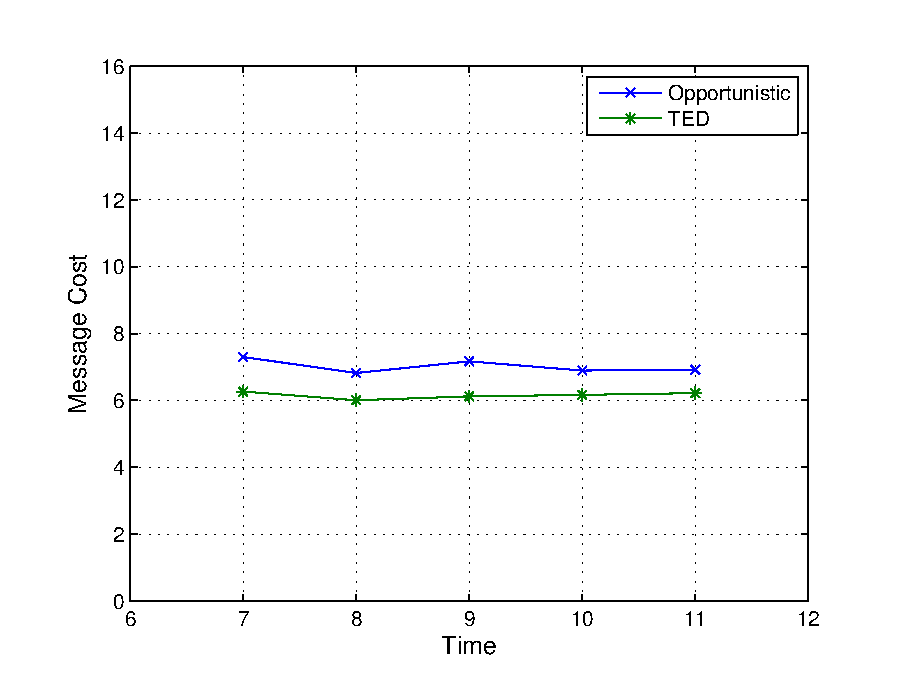
\includegraphics[width=.5\textwidth]{indoorResult1}}
%\qquad
\subfloat[With even fusion point deployment]{\label{fig:indoorResult2}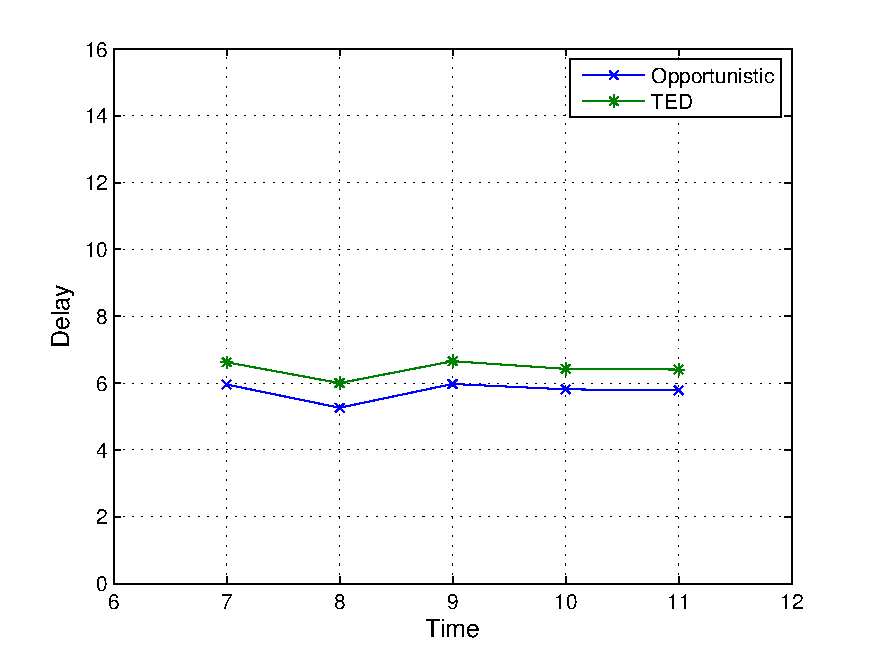
\includegraphics[width=.5\textwidth]{indoorResult2}}
\caption{Experiments for temperature monitoring}
\label{fig:indoorResult}
\end{figure}

\section{Conclusion}
\label{sec:conclusion}
In this paper, we presented PSWare, a flexible middleware framework for composite events processing. PSWare uses a flexible architecture where different event detection mechanisms may easily integrated. We described the design of PSWare and explained how it can be customized for different applications. Then we gave two examples of using PSWare. The first one implements a more general composite event algorithm while the second one uses an application-specific event detection approach. Based on our implementation, we performed experiments and demonstrate the effectiveness of PSWare for prototyping and performance comparison.

\section*{Acknowledgment}
This work is supported by Hong Kong RGC under CERG grant PolyU5102/08E and Hong Kong Polytechnic University under ICRG grant B-13E.

\bibliographystyle{IEEEtran}
\bibliography{../references/wsn-general,../references/wsn-aggregation,../references/wsn-middleware,../references/wsn-pubsub,../references/edl,../references/pubsub,../references/algorithms,../references/event-detection,../references/pervasive}
\end{document}